
\section*{Our code implementation }
Is the code easy-to-use and interpretable? Could you run it?
The code has been written in Python , while back in 2016 the researcher 
decided to write the code for training the Net in LUA .
So first of all we understand the code written in LUA by the authors and 
after we decide to translate it in Python . 
The main reason why we do it is that the code was deprecated after about 10 years (
especially the library ) and for us was not possible to try to train the Net 
ourself . 
Talking about the Datasets they were also not reacheable because the hyperlink redirect 
to a website not existing anymore .
So we try to develop a solution in which we train the Net with the same concept described 
before but using different Datasets .  
Also the trained weights cannot be adapted to the new solution that we develop ,
so we decide so re-train the Network from zero for about 200 epochs .
After the 200 epochs we decide to stop the training because it was taking too long .
\\
The code in subdivided in different part and diffent .ipynb file .
The first one is "1) dataset usage.ipynb" in which is possible the are two example 
on how to load Bird and Flowers Dataset using the module "gan\_t2i" and store it in HDF5 format 
other than using a Dataloader on this datasets .
The second file is "2) CLIP - Fine Tuning.ipynb" in which is shown how to load the CLIP model 
(ViT-B/32) and to train it (we use an already trained CLIP network to extract text features )
The Third file is "3.2) COLAB GAN example.ipynb" . In this file we combine all the 
module that we develop until now . 
First of all we decide which network we would like to train between : "Vanilla\ GAN", "GAN\_INIT\_CLS" 
and "WGAN" . 
After this part we download the weights related to the CLIP Network used to extract 
the text features and also the model itself .
What about the Dataset initially it is stored in HDF5 format but this time is also 
transformed and normalized other than tokenized .
After this section we create the training, validation and test dataloaders and check the 
outcome size of the CLIP model feature related to text and images .
And then depending on the Newtwork that we would like to train 
we define it and define the embedding projection dimension that in our case is 128 .
Finally after this long pre-processing and initilization part we can decide if start to train
the Net using the correspondent Algoritm from zero or from a specific checkpoint ( which corrispond
to the weights ) loading it in the Model . 
The result on the GAN model after 186 epochs of training from scratch are not enough to prodoce a result 
which correspond to the description given by the text , that's due to the fact that the Net is too complex 
and in fact to achieve a satisfactory result, at least 600 epochs are necessary, 
as the original paper also specifies.
Besides the visualization factor it's possible to observe that the loss related to the Discrimination and 
Generator part tend to move in the right direction , in fact the Generator loss especially in the WGAN model
tend do descrease (minimize) and the Discriminator loss it's maximizing it's values as well as described 
in the Min-Max optimization formula .
\\
We try also to conduce some experiments on training the Net addressing the problem to other Datasets 
such as Fashion MNIST dataset ( keras.datasets.fashion\_mnist ) .
Each sample in this dataset is a 28x28 grayscale image associated with a 
label from 10 classes (e.g. trouser, pullover, sneaker, etc.) .
The Net we use was the Wasserstein GAN (WGAN) with Gradient Penalty (GP) which is composed of a Generator 
and a Discriminator Part with different Convolutional Block and Upsampling Block and use the 
Algorithm 2 described in the section related to the Architectures.
\\
In particular the main function used to train the Net is the 
the "train step function" that train the Discrimator first for a fixed 
number of iteration as suggested by the paper .
In this training part for each batch size it create the latent vector , 
create fake images with the generator Net , discriminate between the 
real images and the generated ones and after compute the discrimination 
loss as the difference between the mean of the real and fake logits 
( ouputs of the Discriminator Net ) .
After that the algorithm compute the gradient penalty computing the norm 
of the gradient based on the real interpolated and fake images .
Finally we can compute the discriminator loss adding the penalty term 
and use the choosen optimizer ( ADAM ) to compute the gradient 
descent and backpropagation . 
\\
The last section of the training step implies train the Generator Network.
In this part we don't have to iterate multiple times but is enough to 
create a latent vector , generate the images based on the vector , 
discriminate over the generated images to obtain the logits and 
finally compute the generator loss which is simply the mean of the 
values on the logits vector with negative sign .
As last thing the weight are updated using the generator optimizer 
and computing the gradient .
\\
\begin{figure}[h!]
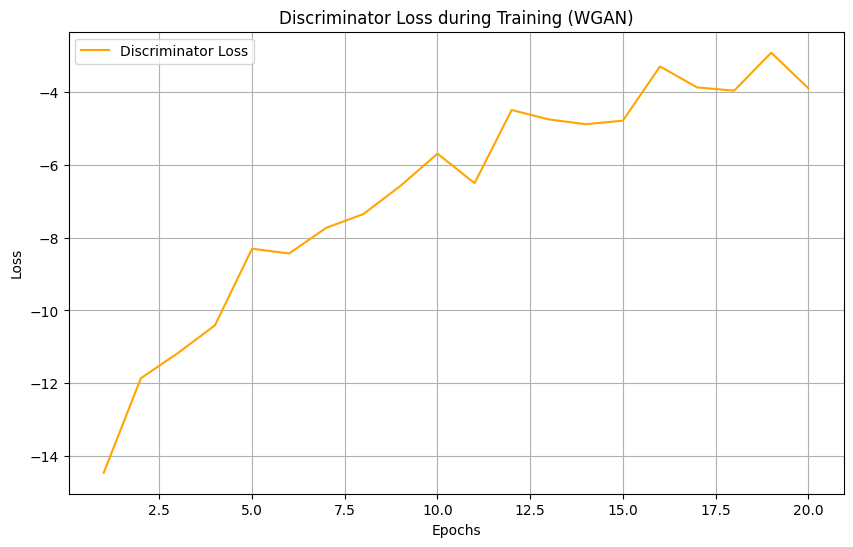
\includegraphics[width=80mm]{D_loss.png}
\caption{Discriminator Loss during Training (WGAN)}
\end{figure}
\\
In general , especially because the problem has been simplified with respect 
to the previous one , after only 50 epochs we can appreciate good result in term of 
reconstruction of image related to the MNIST datasets .
And thanks to the gradient penalty term we can generalize the enough to obtain 
a good reconstruction also on "zero-shot" data coming from the same dataset . 
\\
Add example good reconstruction results .
